\pdfoutput=1

\documentclass[numberedappendix,apj]{emulateapj}
\usepackage{apjfonts}
\usepackage[colorlinks=true,urlcolor=blue,linkcolor=blue,citecolor=blue]{hyperref}
\usepackage{amsmath}
\usepackage{natbib}
\usepackage{graphicx}
%\usepackage{subcaption}

\special{papersize=8.5in,11in}
\setlength{\pdfpageheight}{\paperheight}
\setlength{\pdfpagewidth}{\paperwidth}

% This patch fixes the behavior of the hyperref package to 
% produce ApJ style citations, namely to only highlight the
% year in citecolor = blue rather than the entire citation.

\usepackage{etoolbox}
\makeatletter
% Patch case where name and year have no delimiter
\patchcmd{\NAT@citex}
  {\@citea\NAT@hyper@{\NAT@nmfmt{\NAT@nm}\NAT@date}}
  {\@citea\NAT@nmfmt{\NAT@nm}\NAT@hyper@{\NAT@date}}
  {}% Do nothing if patch works
  {}% Do nothing if patch fails
% Patch case where name and year have basic delimiter
\patchcmd{\NAT@citex}
  {\@citea\NAT@hyper@{%
     \NAT@nmfmt{\NAT@nm}%
     \hyper@natlinkbreak{\NAT@aysep\NAT@spacechar}{\@citeb\@extra@b@citeb}%
     \NAT@date}}
  {\@citea\NAT@nmfmt{\NAT@nm}%
   \NAT@aysep\NAT@spacechar%
   \NAT@hyper@{\NAT@date}}
  {}% Do nothing if patch works
  {}% Do nothing if patch fails
% Patch case where name and year are separated by a prenote
\patchcmd{\NAT@citex}
  {\@citea\NAT@hyper@{%
     \NAT@nmfmt{\NAT@nm}%
     \hyper@natlinkbreak{\NAT@spacechar\NAT@@open\if*#1*\else#1\NAT@spacechar\fi}%
       {\@citeb\@extra@b@citeb}%
     \NAT@date}}
  {\@citea\NAT@nmfmt{\NAT@nm}%
   \NAT@spacechar\NAT@@open\if*#1*\else#1\NAT@spacechar\fi%
   \NAT@hyper@{\NAT@date}}
  {}% Do nothing if patch works
  {}% Do nothing if patch fails
\makeatother

\setcounter{figure}{0}

\graphicspath{{./figs/}}

\begin{document}

%%%%%%%%%%%%%%%%%%%%%%%%%%%%%%%%%%%%%%%%%%%%%%%%%%%%%%%%%%%%%%%%%%%%%
% HEADER:
%%%%%%%%%%%%%%%%%%%%%%%%%%%%%%%%%%%%%%%%%%%%%%%%%%%%%%%%%%%%%%%%%%%%%

\shorttitle{Finding Splashback Radii in Cosmological Simulations}
\shortauthors{Mansfield, Kravtsov, Diemer}

\title{Finding Splashback Radii in Cosmological Simulations}

\author{Philip Mansfield\altaffilmark{1,2,$\star$}, Andrey V. Kravtsov\altaffilmark{1,2,3} and Benedikt Diemer\altaffilmark{4}}

\keywords{ cosmology: theory -- dark matter -- methods: numerical }

\altaffiltext{1}{Department of Astronomy \& Astrophysics, The University of Chicago, Chicago, IL 60637 USA}
\altaffiltext{2}{Kavli Institute for Cosmological Physics, The University of Chicago, Chicago, IL 60637 USA}
\altaffiltext{3}{Enrico Fermi Institute, The University of Chicago, Chicago, IL 60637 USA}
\altaffiltext{4}{Institute for Theory and Computation, Harvard-Smithsonian Center for Astrophysics, 60 Garden St., Cambridge, MA 02138, USA}
\altaffiltext{$\star$}{mansfield@uchicago.edu}

%%%%%%%%%%%%%%%%%%%%%%%%%%%%%%%%%%%%%%%%%%%%%%%%%%%%%%%%%%%%%%%%%%%%%
% ABSTRACT:
%%%%%%%%%%%%%%%%%%%%%%%%%%%%%%%%%%%%%%%%%%%%%%%%%%%%%%%%%%%%%%%%%%%%%

\begin{abstract}

The splashback radius is a drop in the outer density profile of dark matter
halos caused by particles on the apocenters of their first orbit.
This feature has recently gained interest as a physically motivated halo
boundary. However, up to this point all analysis of the splashback radius has
been done on stacked, radially averaged profiles which fail to account for the
large variance and asphericity of this feature. In this paper we present the
code Shellfish (SHELL Finding In Spheroidal Halos) which can identify the full
3D shape of these shells quickly for individual halos from a single particle
snapshot.

\end{abstract} 

\section{Introduction}
\label{sec:introduction}

Placeholder text.

\section{Methods}
\label{sec:methods}

Placeholder text.

\begin{figure}
   \centering
   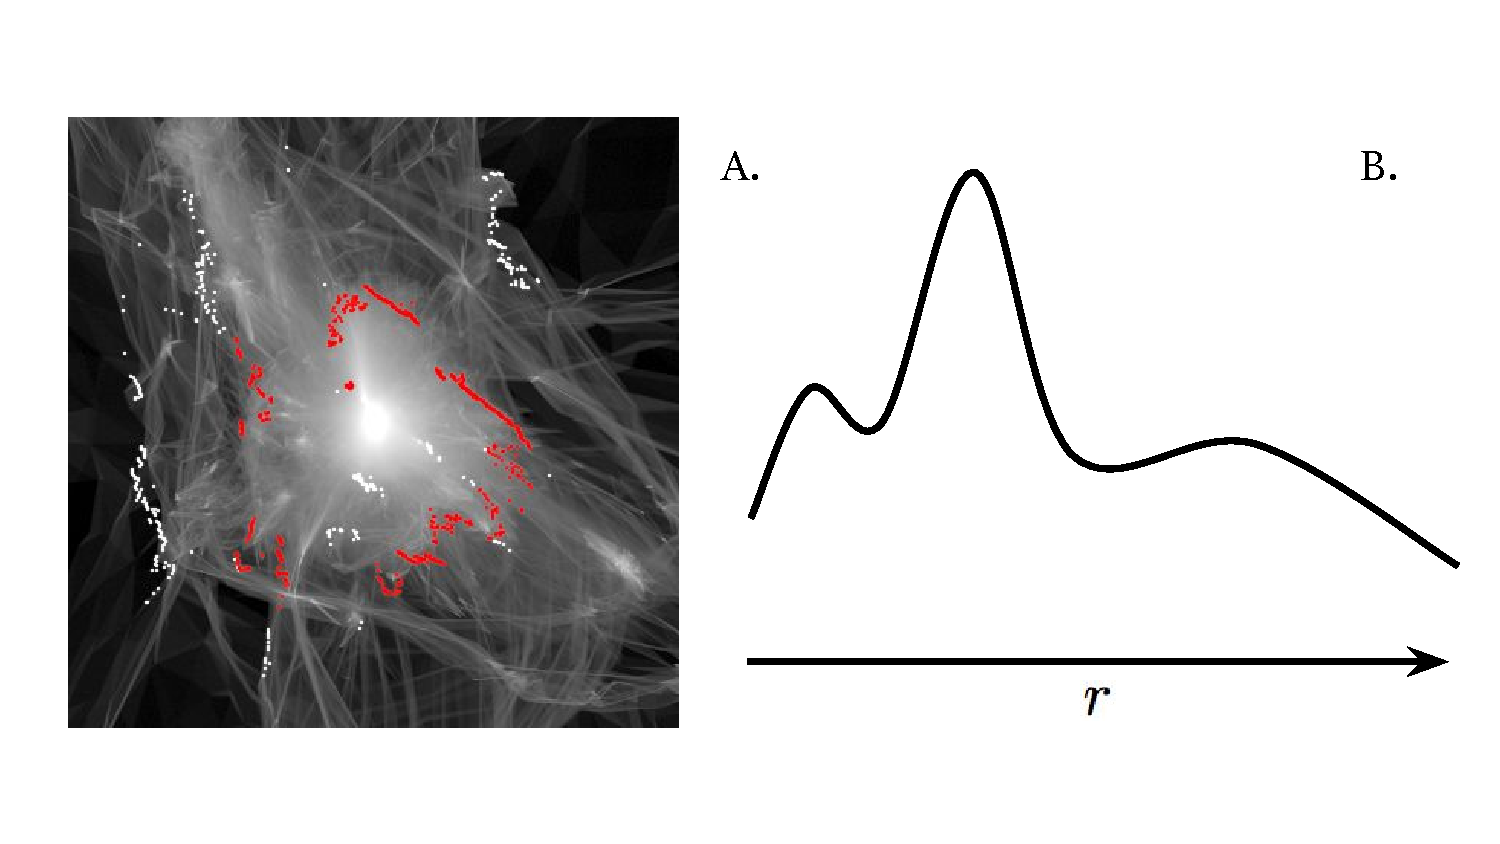
\includegraphics[width=\columnwidth]{shell_finder_algo_a.pdf} \\
   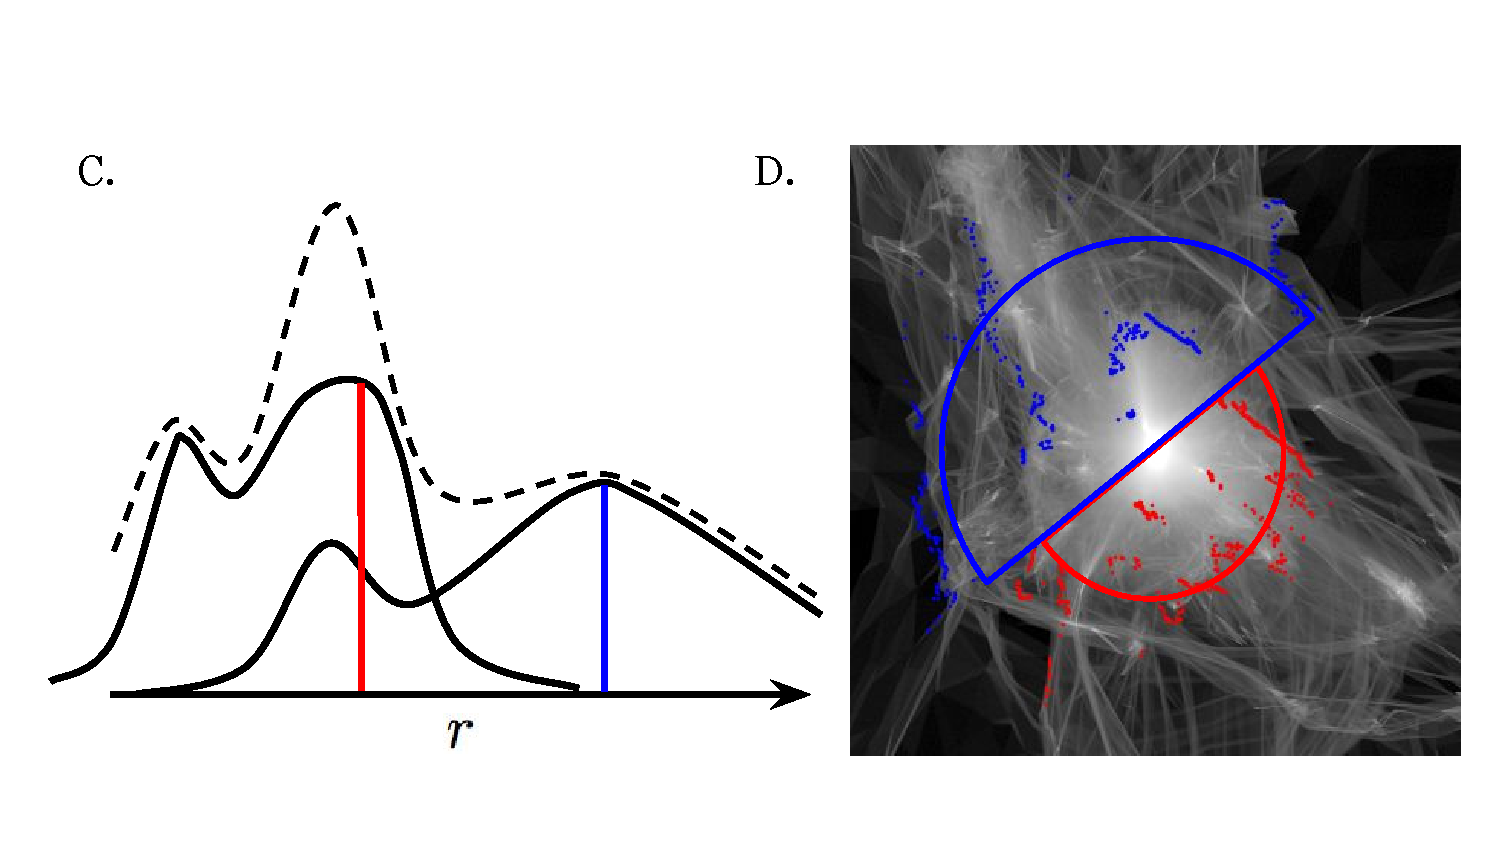
\includegraphics[width=\columnwidth]{shell_finder_algo_b.pdf}
   \caption{An illustration of Shellfish's filtering algorithm. Panel A shows
      a slice through the density field of a halo with the points of steepest
      slope along 1024 uniformly spaced lines of sight shown as red and white
      dots. For this halo, there are three populations of dots: those which
      correspond to the splashback shell (roughly shown in red), those which
      correspond to subhalos within the splashback shell and those which
      correspond to filaments outside the splashback shell. A cartoon
      representing the distribution of radii is shown in panel B.
      \textcolor{red}{\textbf{TODO: Flip C and D, make less ugly. Make caption
      shorter.}}
   }
   \label{fig:shell_finder_algo}
\end{figure}

\begin{figure}
   \centering
   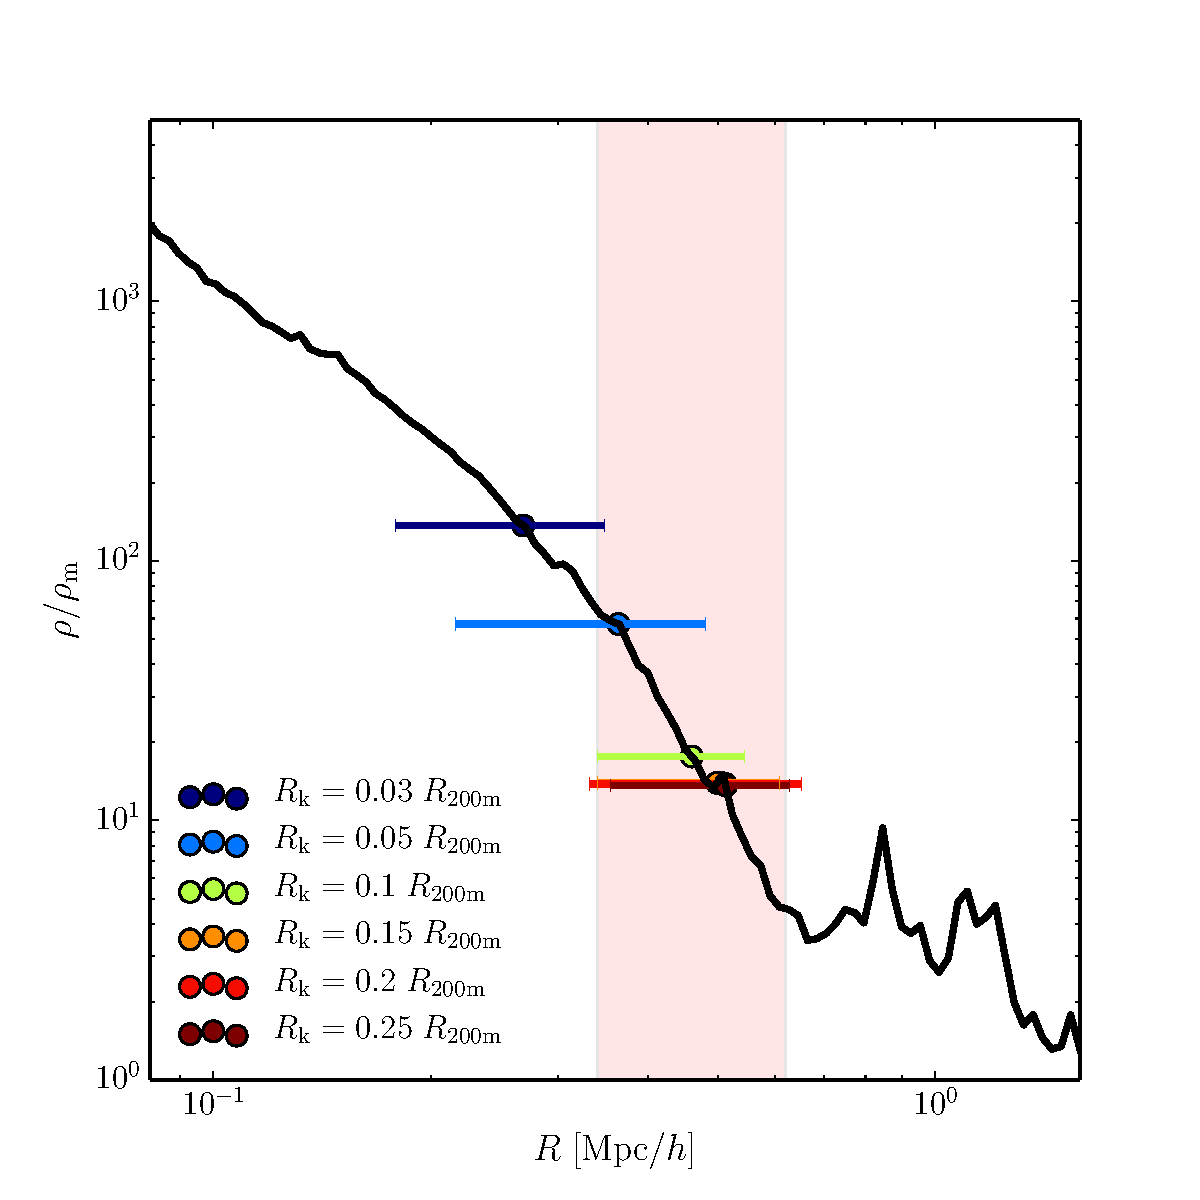
\includegraphics[width=\columnwidth]{rk_convergence_prof.pdf}
   \caption{Convergence test of $R_{\rm sp}$ as a function of kernel radius for
      a representitive halo. The black curve is the density profile of the halo,
      the points are the $R_{\rm sp}$ values measured at different kernel radii,
      the horizonal lines show the range spanned by $R_{\rm min}$ and
      $R_{\rm min}$ for these shells, and the shaded red region corresponds to
      the radial range which was visually identified as corresponding to the
      splashback range. This region was found without knowledge of the
      measurments made by Shellfish in accordance with the procedure outlined
      in Appendix \ref{sec:visual}. For this halo, $R_{\rm sp}$ is converged
      for kernel radii above $0.15R_{\rm k}$
   }
        \label{fig:rk_convergence_prof}
\end{figure}

\begin{figure}
   \centering
   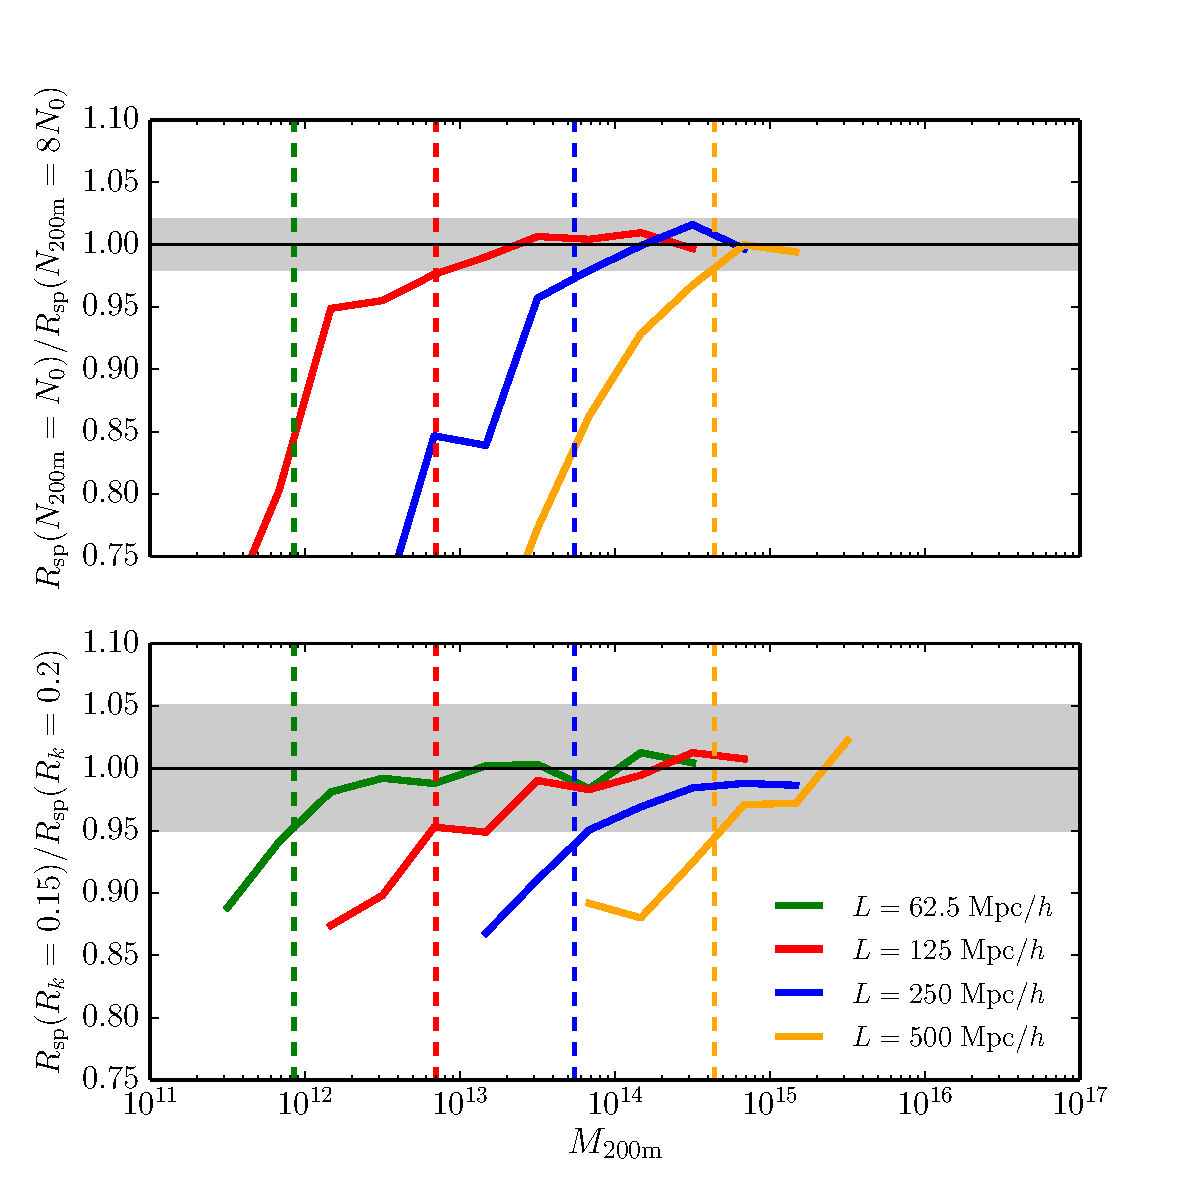
\includegraphics[width=\columnwidth]{m200_rsp_convergence.pdf}
   \caption{Convergence test of $R_{\rm sp}$ with $N_{\rm 200m}$. The top panel
       shows the median ratio of $R_{\rm sp}$ to the value of $R_{\rm sp}$ that
       would be measured if that halo was resolved with 8 times the resolution
       for halos of a given mass in each simulation in our suite. This value
       is simulated by comparing subsampled and fully sampled halos from a
       a more finely resolved simulation. The bottom panel shows the median
       ratio of $R_{\rm sp}$ measured with kernel radii of
       $R_{\rm k} = 0.15 \times R_{\rm 200m}$ to $R_{\rm sp}$ measured with
       kernel radii of $R_{\rm k} = 0.20 \times R_{\rm 200m}$. The vertical
       lines show the masses at which $N_{\rm 200m} = 5 \times 10^4$ in
       each simulation, and the shaded gray regions show the size of 2\% and
       5\% deviations for the upper and lower panels, respectively. The top
       panel uses kernel sizes of $R_{\rm k} = 0.20 \times R_{\rm 200m}$.
       The top panel demonstrates that a systematic offset of $\gtrsim 2\%$ can 
       be expected at $N_{\rm 200m} < 5\times 10^4$. The bottom panel
       demonstrates that the particle counts which correspond to a 2\% reduction
       in radius under subsampling result in a 5\% reduction in radius under
       kernel size reduction. The significance of this alignment is discussed
       in the text. (\textcolor{red}{\textbf{This is likely to be confusing.}})
   }
        \label{fig:m200_rsp_convergence}
\end{figure}

\begin{figure*}
   \centering
   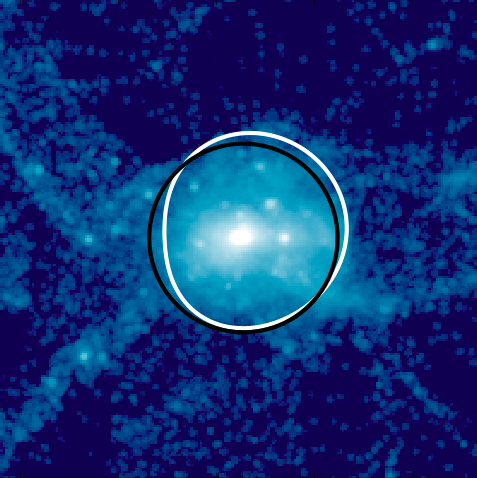
\includegraphics[width=0.7\columnwidth]{example_halos/pass_ex1.png}
   \hspace{0.4cm}
   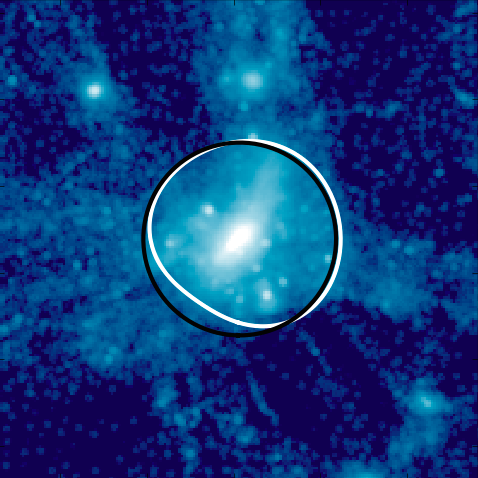
\includegraphics[width=0.7\columnwidth]{example_halos/pass_ex2.png}\\
   \vspace{0.5cm}
   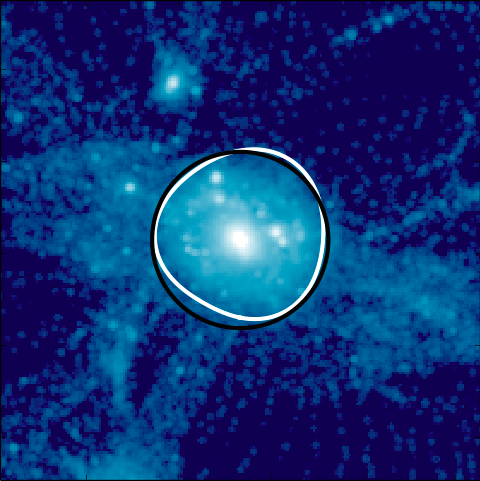
\includegraphics[width=0.7\columnwidth]{example_halos/pass_ex3.png}
   \hspace{0.4cm}
   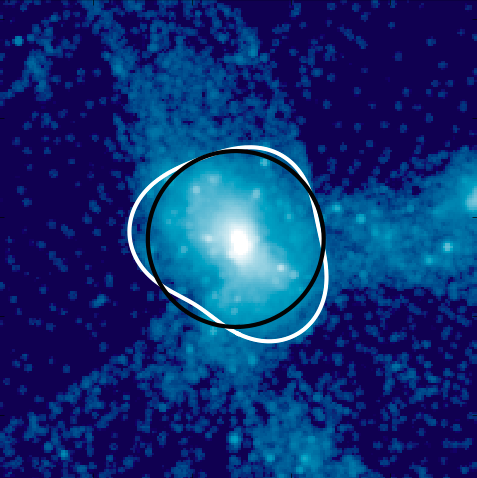
\includegraphics[width=0.7\columnwidth]{example_halos/pass_ex4.png}\\
   \vspace{0.5cm}
   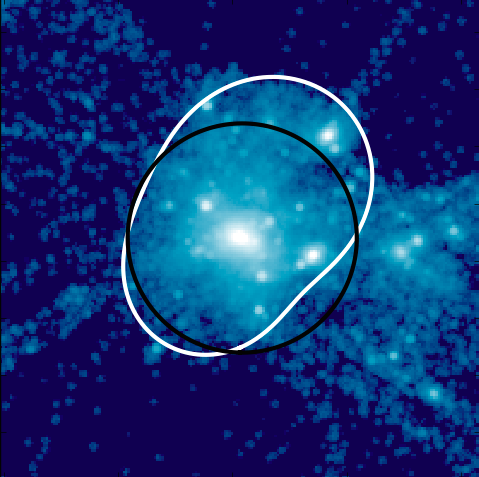
\includegraphics[width=0.7\columnwidth]{example_halos/pass_ex5.png}
   \hspace{0.4cm}
   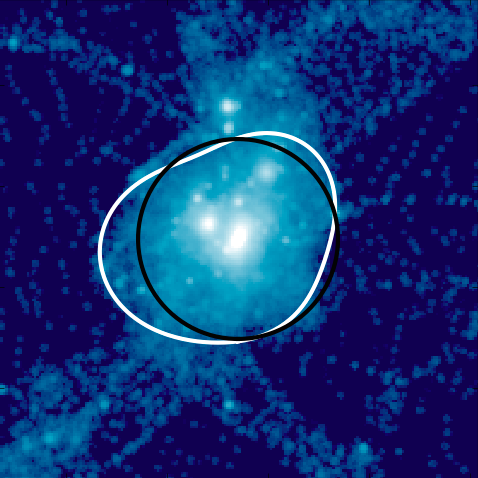
\includegraphics[width=0.7\columnwidth]{example_halos/pass_ex6.png}
   \caption{Density slices of six randomly selected halos compared to the
      shells measured by Shellfish. The shape of the shell within this slice
      is shown by the white curve and the a sphere with the same
      volume as the shell is shown in black. The six halos were picked uniformly
      from the $\log{M_{\rm 200m}}-\log{\Gamma}$ plane in out \texttt{L0063}
      simulation box and are each plotted out to $2.5 R_{\rm 200m}$.}
      \label{fig:pass_ex}
\end{figure*}

\begin{figure*}
   \centering
   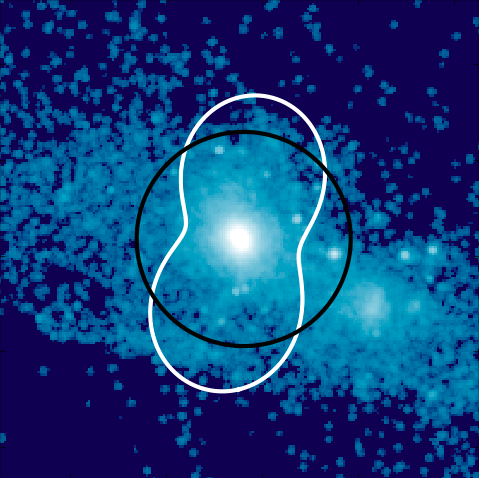
\includegraphics[width=0.7\columnwidth]{example_halos/fail_ex1.png}
   \hspace{0.4cm}
   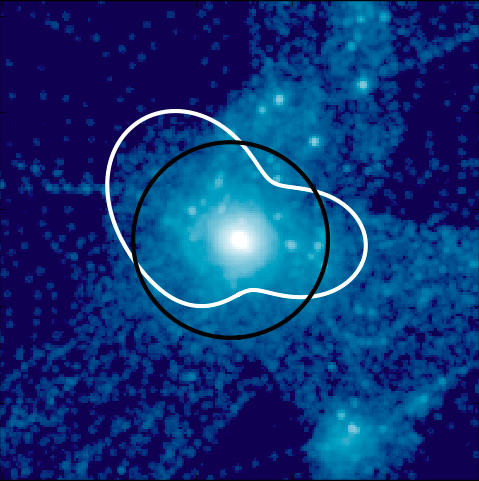
\includegraphics[width=0.7\columnwidth]{example_halos/fail_ex2.png}
   \caption{Examples of halos for which Shellfish produces poor shells. These
        halos were chosen by randomly selecting halos from the population of
        halos which fail the cut described in Appendix \label{sec:visual} until
        two were found which did not appear to be
        good fits by eye. The left panel is typical these types of halos: they
        often inhabit strong filaments and do not contain a visually apparent 
        splashback shell in their dentity fields, although, as demonstrated in
        the right panel, there are some halos with visually apparent splashback
        fields which Shellfish measures incorrectly, too. The right panel also
        demonstrates that even in cases where the full shell is incorrect, the
        volume-equivalent radius can be relatively well-behaved. We estimate
        that Shellfish generates these types of shells for roughly 5\% of the
        halos in our sample.}
        \label{fig:fail_ex}
\end{figure*}

\section{Results}
\label{sec:results}

\begin{figure*}
   \centering
   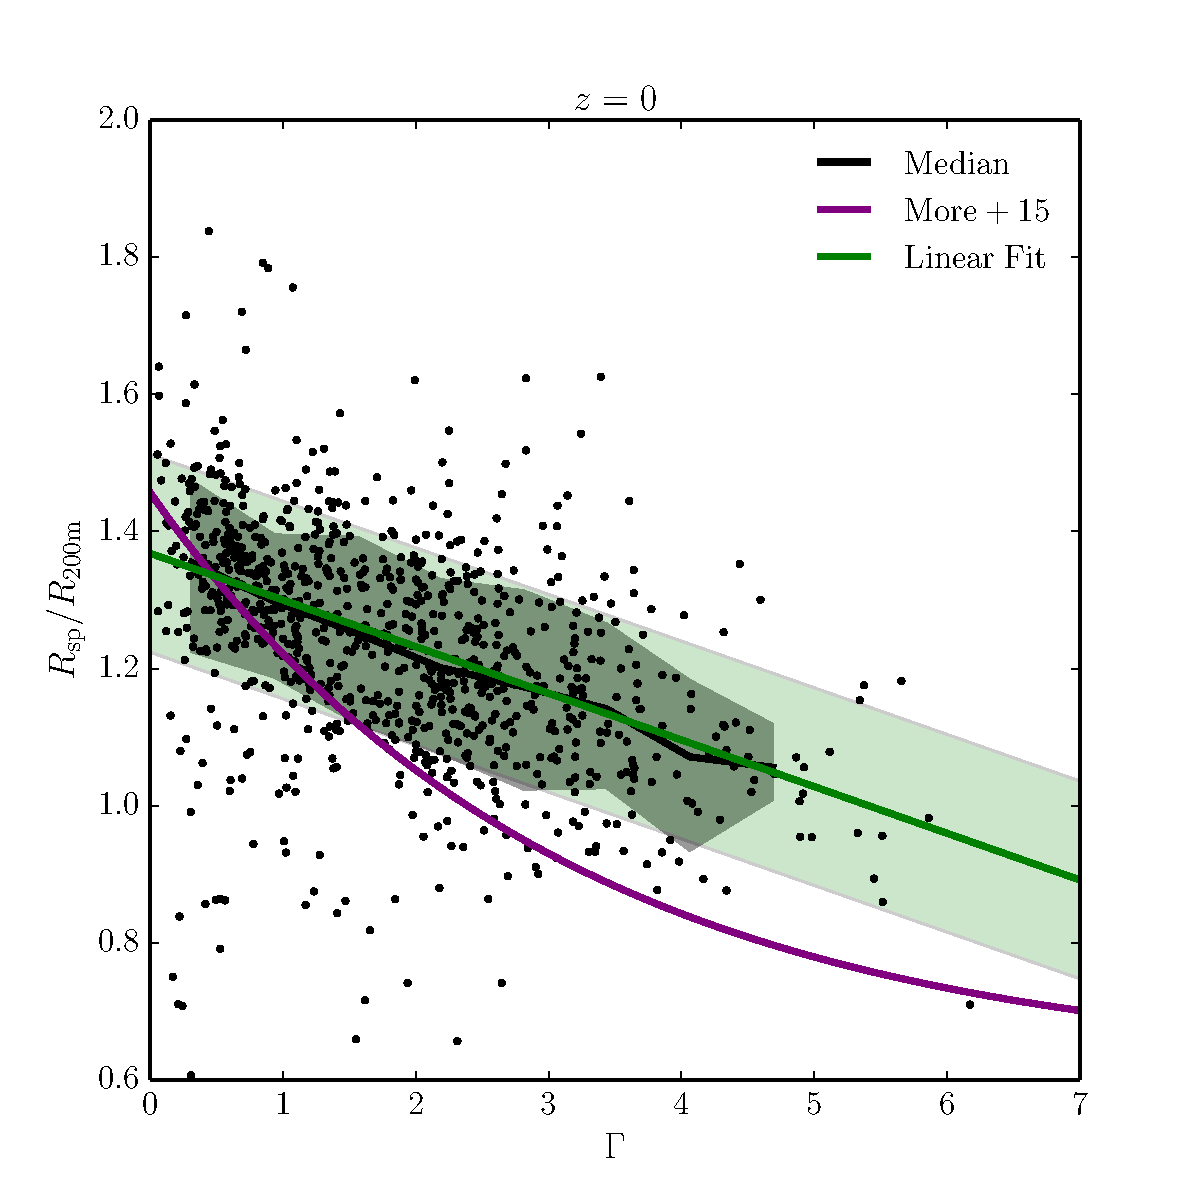
\includegraphics[width=\columnwidth]{z0_fit.pdf}
   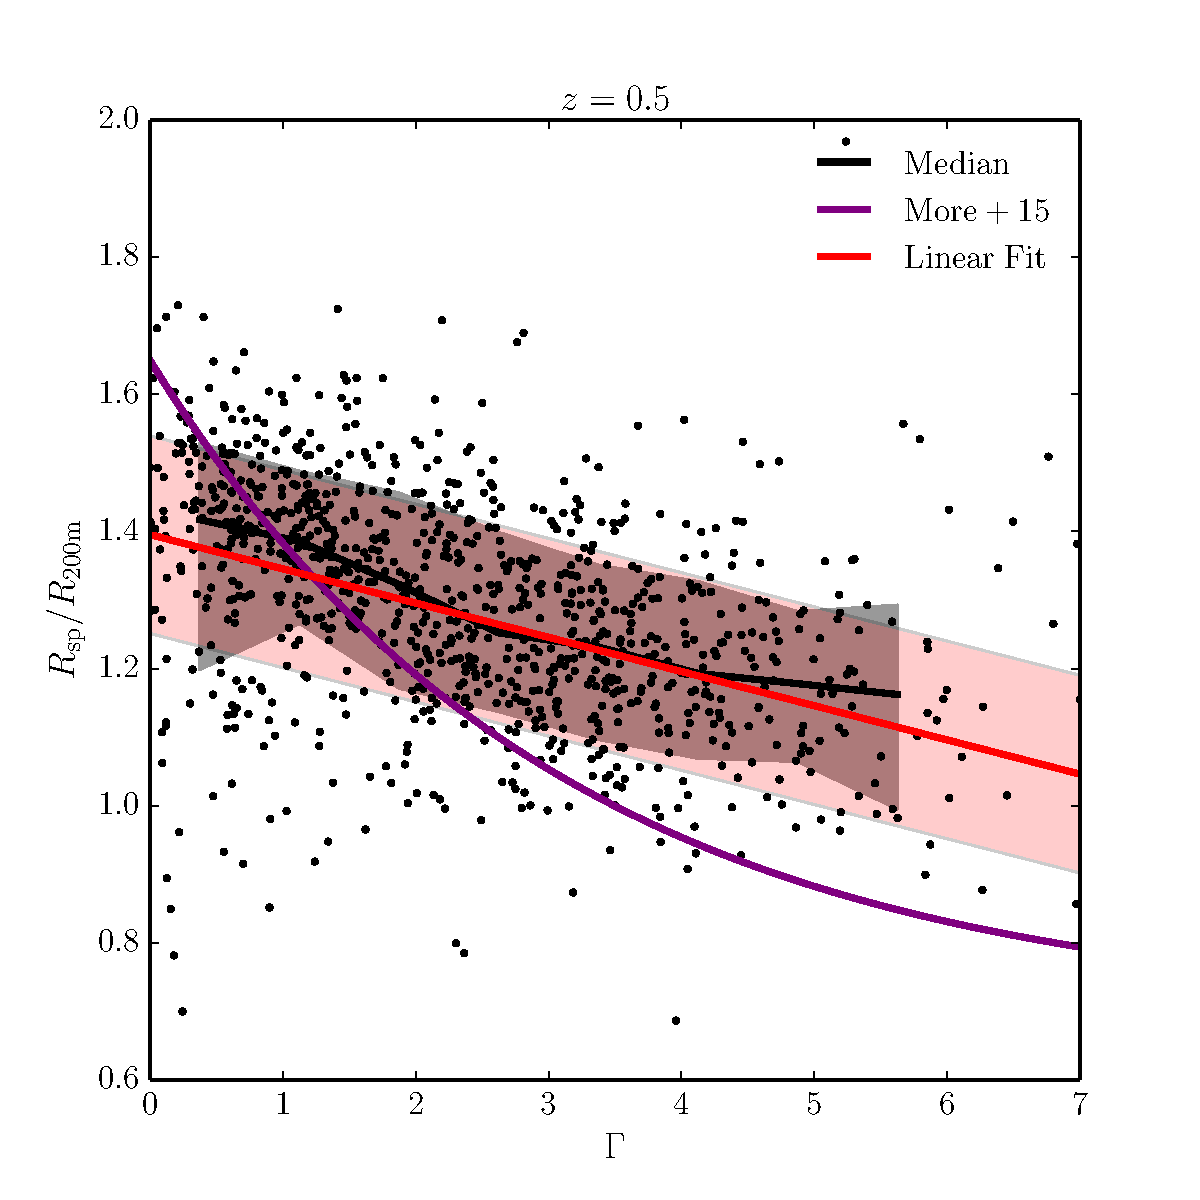
\includegraphics[width=\columnwidth]{z05_fit.pdf}\\
   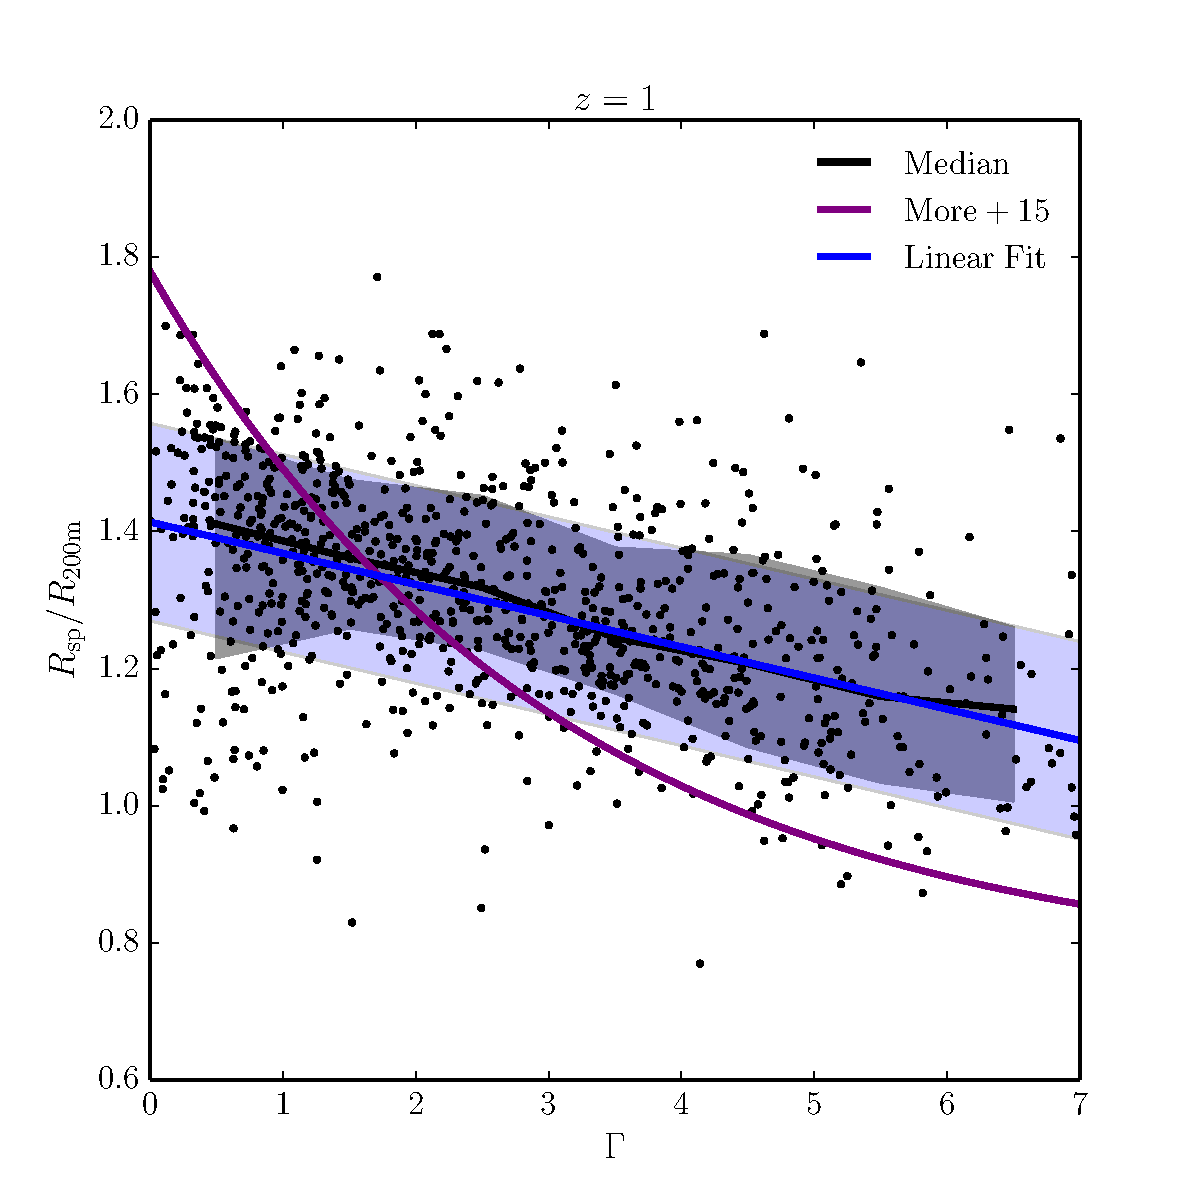
\includegraphics[width=\columnwidth]{z1_fit.pdf}
   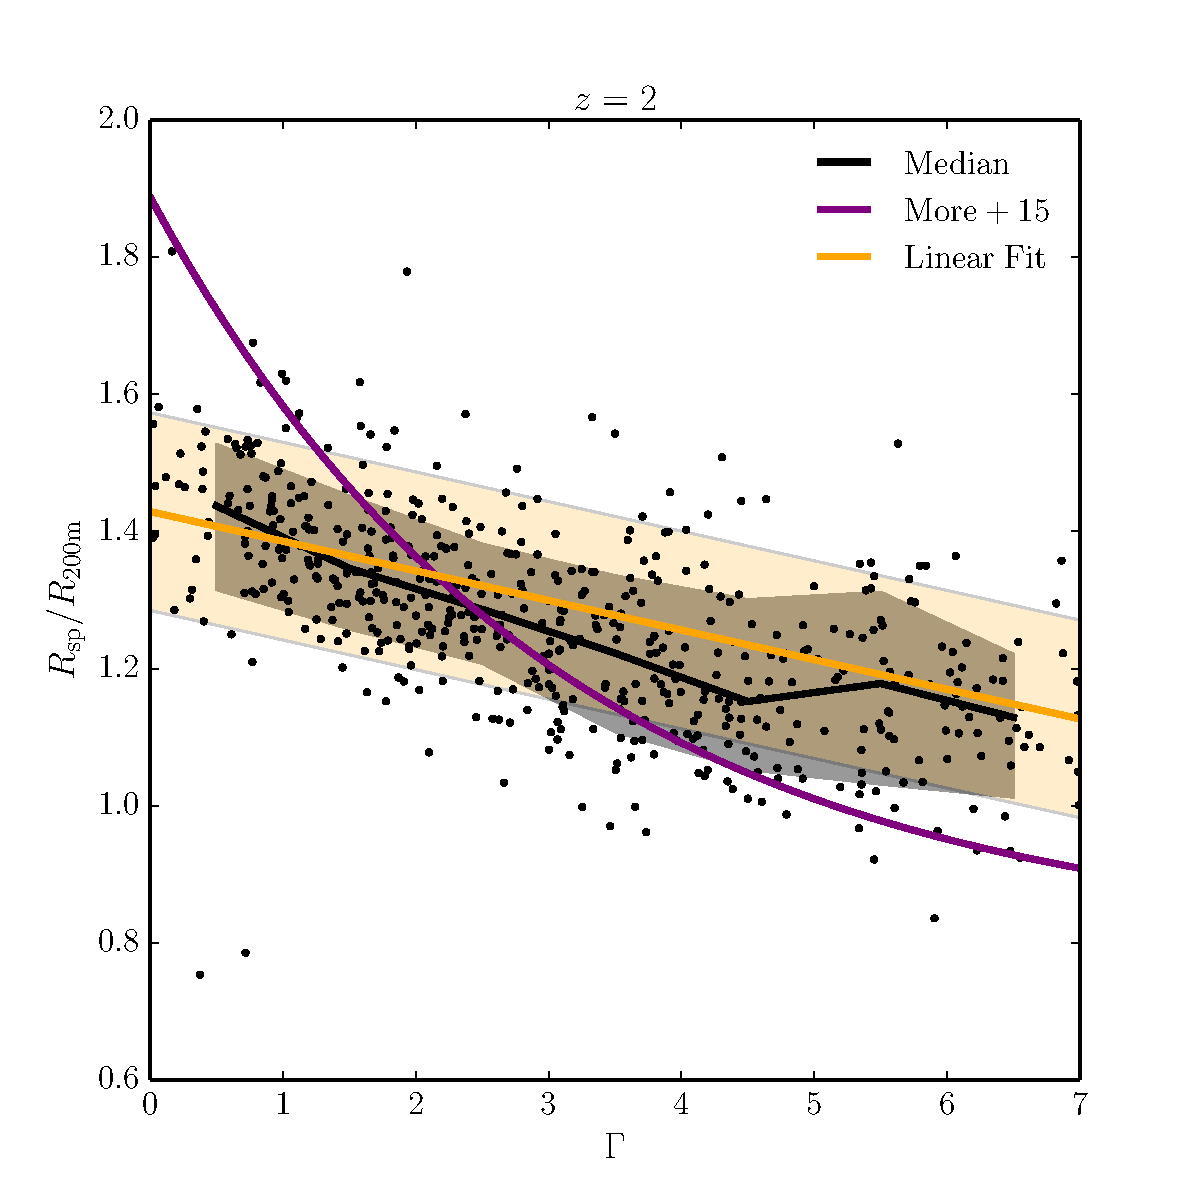
\includegraphics[width=\columnwidth]{z2_fit.pdf}
   \caption{The $R_{\rm sp}/R_{\rm 200m}$ vs. $\Gamma$ relation as measured
        by Shellfish. The points are individual halos, the black curves and gray
        shaded regions are the medians and the 68\% envelopes of the point
        distributions, respectively. The colored curves and shaded regions are
        the peak and 1$\sigma$ tails of the fitted distribution given by
        (\textcolor{red}{\textbf{insert reference}}). The purple curve is the
        relation given in \citet{more_et_al_2015}, which is found by finding the
        point of steepest slope of stacked profiles. The two families of curves
        are different in both shape and amplitude.}
        \label{fig:z_fit}
\end{figure*}

Placeholder text.

\section{Discussion}
\label{sec:discussion}

Placeholder text.
 
\section{Summary and conclusions}
\label{sec:summary}

Placeholder text.

\acknowledgments

Placeholder text.

\bibliographystyle{apj}
\bibliography{splashback}

\appendix

\section{An algorithm for fast LOS density measurements}
\label{sec:intersection}

The first step of Shellfish's shell-finding algorithm is to assign densities to
a large number of lines of sight anchored the center of each halo. In the case
where density estimates are constructed by converting particles into a set of
volume-filling constant density convex solids (such as spherical top hat kernels
or constant density tetrahedra under the method of \citealt{abel_et_al_12}), the density along a line of sight, $l$, is
\begin{equation}
        \label{eq:los-rho}
        \rho_l(r) = \sum_{i=0}^{i<N}\mathbb{I}_{\rm intr}\rho_i
        H(r - r_{\rm in})H(r_{\rm out} - r),
\end{equation}
where $i$ indexes over all the solid, $\mathbb{I}_{\rm intr}$ is an indicator
function which is 1 if the solid intersects with solid $i$ and 0 otherwise,
$\rho_i$ is the density of this solid, $H$ is the Heaviside step function, and
$r_{\rm in}$ and $r_{\rm out}$ are the distances to entrance and exit
intersection points, respectively.

For a typical choice of density estimator the number of zero terms in
Eq.~\ref{eq:los-rho} dwarfs the number of non-zero terms, making efficient
evaluation of $\mathbb{I}_{\rm intr}$ critical. This is trivial if a density
estimate is written to an intermediate grid before being translated onto the
lines of sight, since the grid cell that corresponds to the point
at radius $r$ of given ray can be calculated in $O(1)$. However, using an
intermediate grid has a number of disadvantages:
\begin{enumerate}
        \item[1.] Maintaining the high-resolution grid required to measure
        asphericities in the splashback shell consumes
        a large amount of space. This restricts the number of halos which
        can be maintained in memory at once. In the case where a user requests
        analysis of more halos than can fit memory at once, Shellfish would need
        to read particle catalogs from disk multiple times.
        \item[2.] Writing the density esitmate to a grid is expensive as it
        involves either an exact raterization scheme (see, for example,
        \citealt{powell_abel_14}) or Monte Carlo sampling of each solid with
        sufficiently many points to elimate shot noise in the estimate. This
        will also require that density estimates are calculated for grid cells
        which are not intersected by any line of sight.
        \item[3.] Introducing an intermediate grid reduces the fidelity of the
        line of sight density estimates due to pixelation. This is most apparent as small
        radii.
\end{enumerate}
In practice we find that these three disadvantages, particularly the second,
make the use of grids undesirable for Shellfish. For this reason, we designed an
algorithn which evaluates Eq.~\ref{eq:los-rho} exactly up to the resolution of
the line of sight profiles without the use of a grid.

\textcolor{red}{\textbf{Preamble goes here. Split up into halos and
rings.}}\footnote{For the purposes of this analysis, it is assumed
that performing an intersection check is also sufficient to evaluate
$r_{\rm in}$ and $r_{\rm out}$. This is true for virtually all solids.}.
For each particle catalog file, the following actions are performed:
\begin{enumerate}
        \item[1.] A bounding box is constructed around the solids creates by
        the particles in the file. An intersection check is performed between
        every analyzed halo and this box. Only the lines of sight which reside
        in halos that pass this check are analyzed further.
        \item[2.] Intersection checks are performed between every halo and
        solid in the catalog file.
        \item[3.] For each halo, the set of intersecting solids is iterated
        over. For each of the halo's rings, perform an intersection check is
        performed between the solid and the plane which the ring is embedded
        within. If this check is successful, the shape corresponding to the 
        intersection between the plane and the surface of the solid is computed.
        \item[4.] The angles of the the upper and lower edges of the shape
        are calculated relative to the center of the halo along the
        corresponding plane. This identifies eactly the set of lines of sight
        in this ring which interect the object.
        \item[5.] An intersection check is performed between the solid and these
        lines of sight to calculate $r_{\rm in}$ and $r_{\rm out}$.
        \item[6.] The combined step function is added to the appropriate radial
        profile as shown in Eq.~\ref{eq:los-rho}.
\end{enumerate}

This is illustrated in Fig.~\ref{fig:intr_algo}.

\begin{figure}
\centering
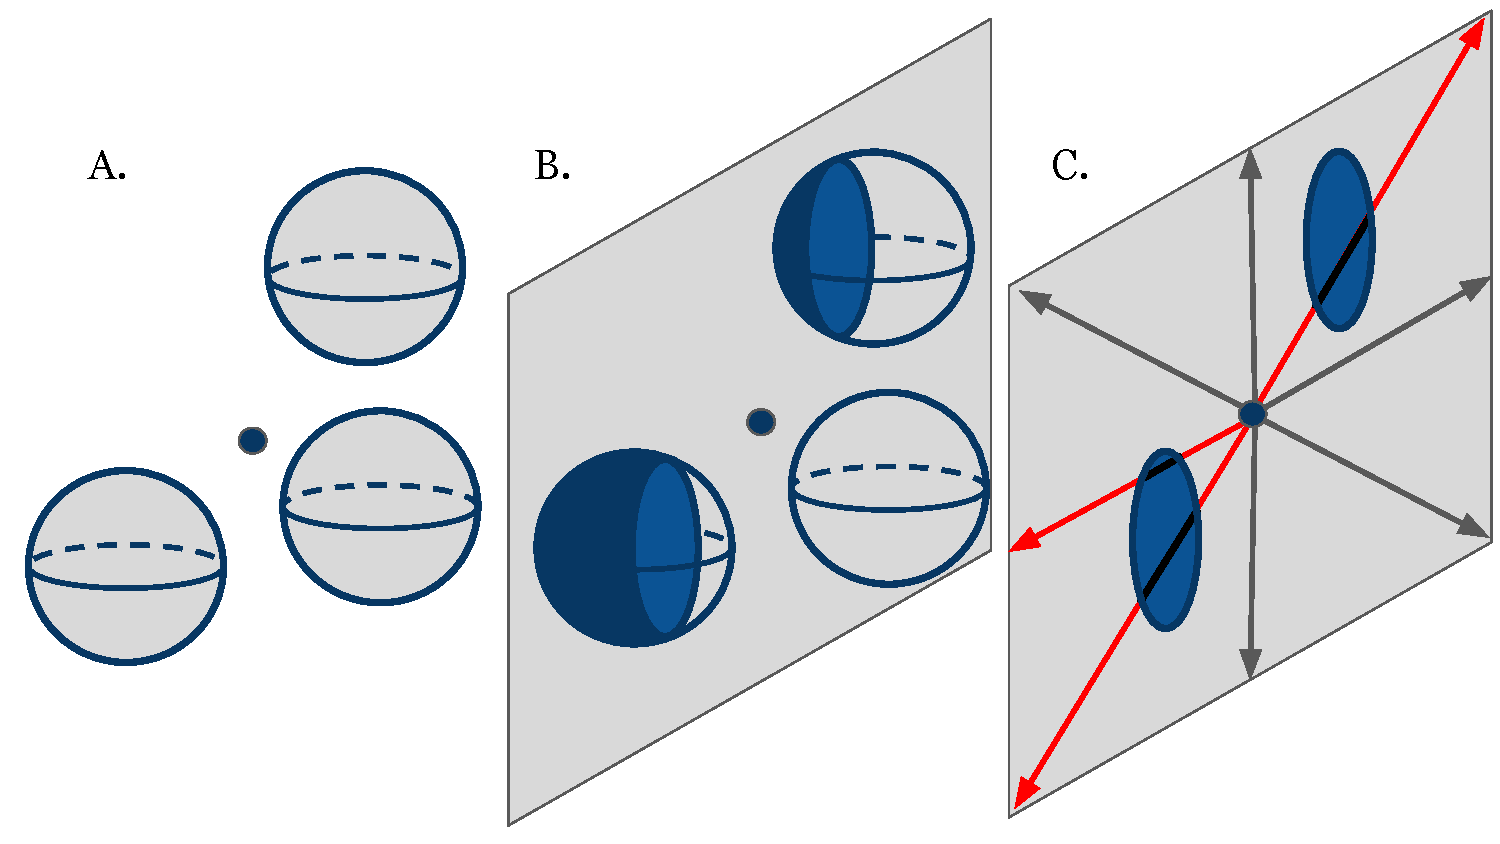
\includegraphics[width=\columnwidth]{intr_algo.pdf}
\caption{An illustration of the algorithm described in this Appendix. Panel A
         shows several spherical kernels oriented around the center of a halo
         which have successfully passed steps 1 and 2 of the algorithm. Panel B
         shows interseciton checks being made on a plane corresponding to a
         ring of line of sight rays. The top and left spheres intersect this
         plane while the remaining sphere does not. This corresponds to step
         3 of the algorithm. Panel C shows intersection checks being performed
         between the 2D slices of the kernels and the lines of sight in the
         ring. Inspection of the angular locations of the edges of these slices
         shows that only the red lines of sight could intersect
         them, meaning that no calculations are performed on the black lines.
         This corresponds to steps 4 and 5 of the algorithm.}
           
\label{fig:intr_algo} 
\end{figure}

The process described above has a number of inefficiencies. The most
important algorithmic optimizations are described below:
\begin{itemize}
        \item The first time step 1 is performed in a given simulation,
        Shellfish writes these bounding boxes to a series of header
        files so that they do not need to be recomputed. 
        \item Shellfish restricts ever halo to have the rings with the same
        set of normal vectors. It performs step 3 by first iterating over
        the set of normal vectors and rotating all the solids into a coordinate
        system in which that normal vector is pointed in the $\hat{z}$
        direction. Since this only needs to be done once across many halos, the
        amortized cost is small and it allows the geometric primitives needed
        in this step to be significantly optimized.
        \item For virtually all solids, it is more efficient to perform an
        intersection check betwen a line and the 2D shape found at the end of
        step 3 than it is to do an intersection check between a ray and the
        solid in 3D. For this reason, step 5 is performed with the former and
        not the latter.
        \item If all other optimizations are performed and step 6 is
        implemented naively, it is the dominating cost in the procedure despite
        its simplicity. For this reason, instead of representing the profiles
        as arrays containing $\rho(r)$, we represent them as arrays containing
        ${\rm d} \rho(r) / {\rm d} r$. This means that every update of the
        profile requires modifying at most four array elements near 
        $r_{\rm in}$ and $r_{\rm out}$. Once every solid has been looped over,
        the profiles are integrated to optain $\rho(r)$.
\end{itemize}

For a system with $N$ solids, $L$ lines of sight, $I$ total intersection points
between all solids and all lines of sight, and $B$ radial bins per profile, a
naive evaluation of Eq.~\ref{eq:los-rho} would require $O(NL)$ intersection
checks and $O(IB)$ updates to density profiles. The algorithm we presented above
performs $O(I)$ intersection checks, $O(I)$ updates to profiles, a
post-processing step which performs $O(LB)$ profile accesses, and a
preprocessing step that performs $O(NR)$ geometric operations, where $R$ is the
total number of rings. Since $L \ll I \ll NL$ and $1 \ll L$,
this corresponds to a reduction in the number of operations by many orders
of magnitude.

\section{Visually identifying splashback radii from density profiles}
\label{sec:visual}

\textcolor{red}{\textbf{(Flesh out this section eventually. Should probably
move to main text.)}}

(Roughly from the most strict to least strict cut.)

(The main purpose of all of these is to rule out splashback regions which are
either created or distorted by suhalos or mergers.)

\begin{itemize}
        \item The halo is not within $R_{\rm 200m}$ of a larger halo.
        \item The halo much have an apparent steepening of both the density
        and subhalo density profiles at the same radial range.
        \item There must not be a ``large'' subhalo
        ($M_{\rm 200m,\ sub} > M_{\rm 200m,\ host}/15$) exactly at the start of
        the steepening region.
        \item There must not be significant subhalo presence in the steepening
        region.
        \item The slope of the steepening region must be steeper than -3.
        \item The concentration of the halo must be greater than 2.
\end{itemize}

\begin{figure}
    \centering
     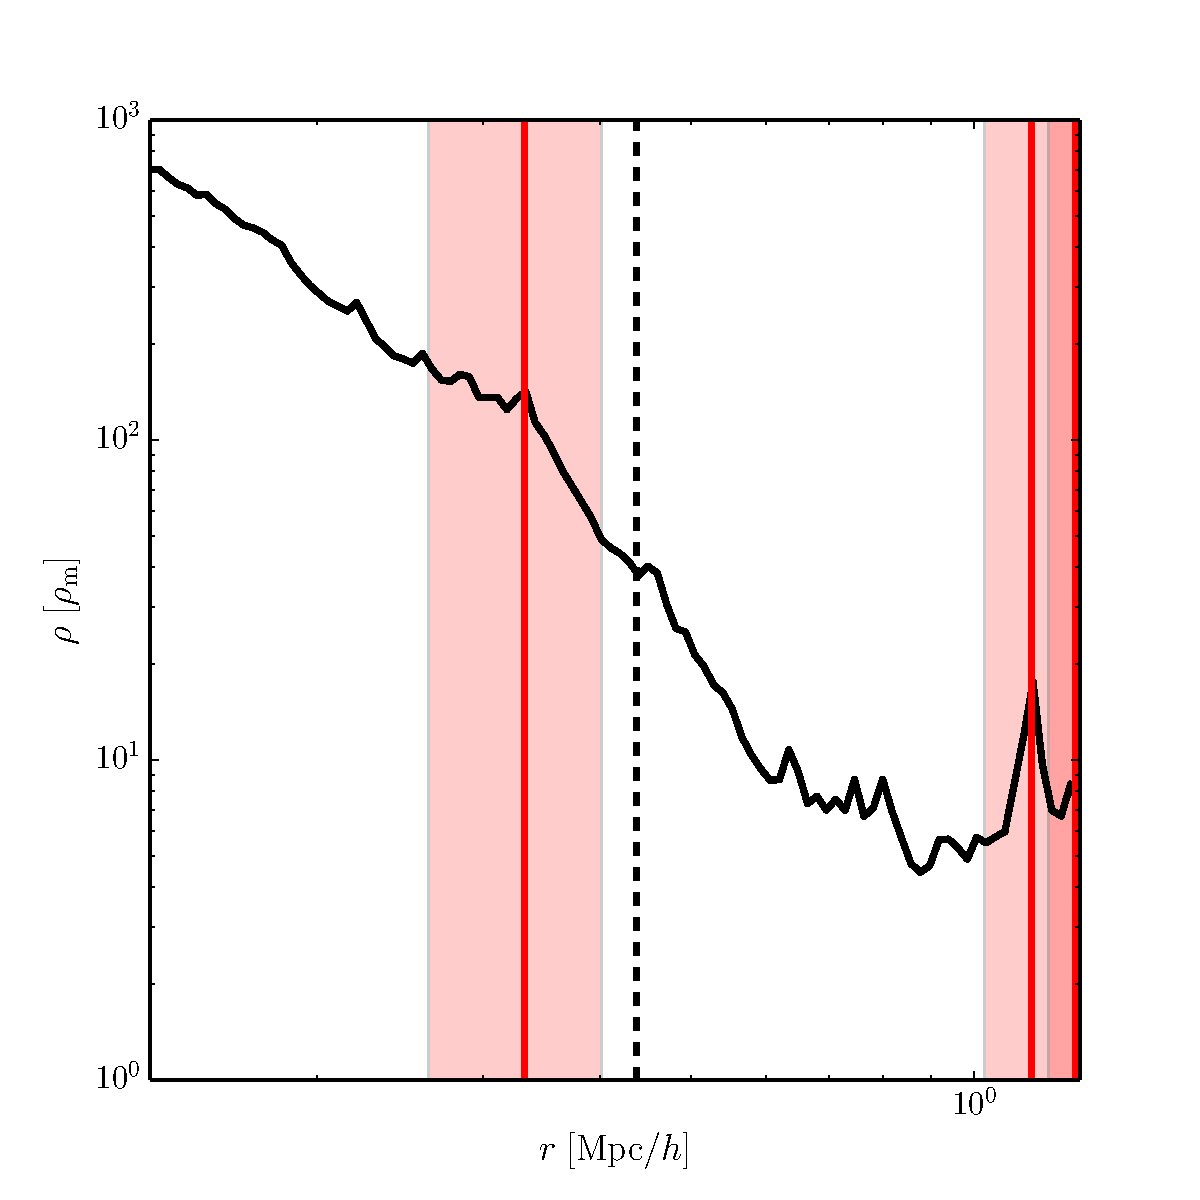
\includegraphics[width=0.4\columnwidth]{subhalo_contamination.pdf}
     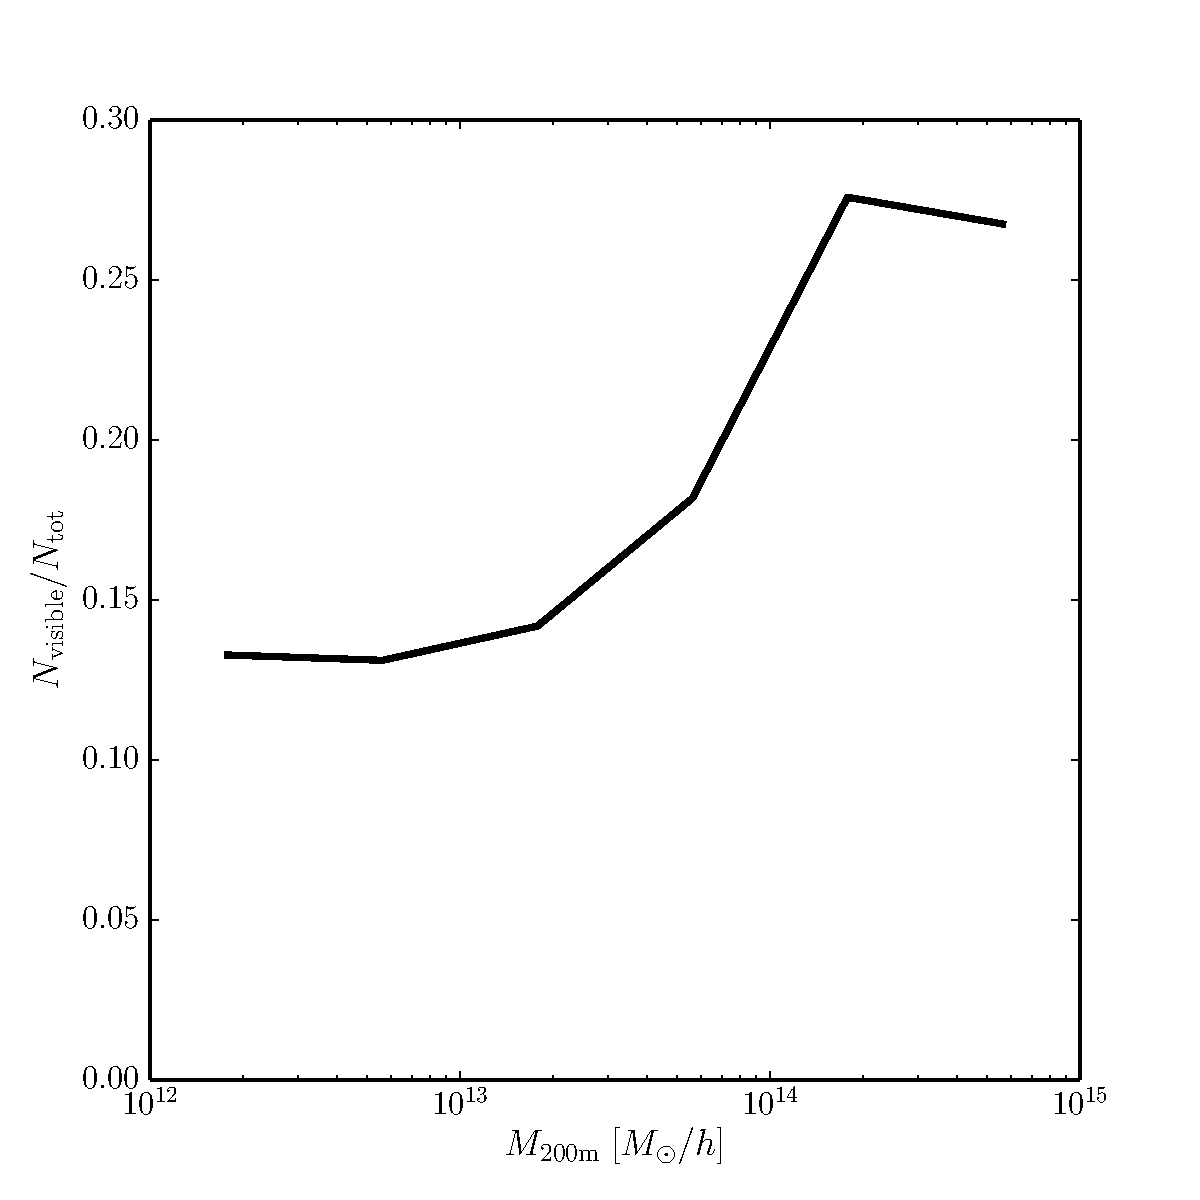
\includegraphics[width=0.4\columnwidth]{vis_frac_m.pdf}
     \caption{\emph{Left:} An example profile of an $M_{\rm 200m}$ =
        $5 \times 10^{12}\ M_\odot/h$ halo which would
        not be included in the set of halos with visually identifiable
        splashback ranges. The plot show a one
        decade window centered around $R_{\rm 200m}$ (shown by the vertical
        dashed line). The vertical red lines show the location of every subhalo
        with $M_{\rm 200m,\ sub} > M_{\rm 200m,\ host} / 15$ and the shaded
        regions correspond to the radial range enclosed by $R_{\rm 500c}$ for
        these halos. This halo would not meet the cut described in this
        Appendix because the apparent start of the splashback zone conicides
        exactly with the peak of a subhalo, making the true start of the
        splashback zone unclear. \emph{Right:} The fraction of halos which pass
        the cuts described in this Appendix as a function of mass. The number
        of such halos increases with increasing mass, but even at the highest
        masses the majority of halos do not meet these cuts.}
     \label{fig:vis_figs}
\end{figure}

\end{document}
